\documentclass[10pt,a4paper]{article}
\usepackage[english]{babel}
\usepackage[utf8]{inputenc}
\usepackage{amsmath}
\usepackage{amsfonts}
\usepackage{amssymb}
\usepackage{graphicx}
\usepackage{float}
\usepackage{caption}

%link to documentation: 
%https://ackrep-doc.readthedocs.io/en/latest/devdoc/contributing_data.html

\begin{document}
	\part*{Model Documentation of the \\ Permanent Magnet DC Motor} % MUST - Add Model Name 
	
	%%%%%%%%%%%%%%%%%%%%%% NOMENCLATURE %%%%%%%%%%%%%%%%%%%%%%%%%%%
	
	\section{Nomenclature} % MUST
	\subsection{Nomenclature for Model Equations} % MUST
	
	%variables for model equations
	\begin{tabular}{ll}
		$c\phi$ & motor constant \\
		$J$ & moment of inertia \\
		$L_A$ & armature inductance \\
		$R_A$ & armature resistance \\
		$i_A$ & armature current \\
		$\omega$ & angular velocity \\
		$u_A$ & armature voltage \\
		$\xi_L$ & load moment \\
				
	\end{tabular}
	 
	
	\subsection{Graphic of the Structure}	
	\begin{figure}[H]
		\centering
		\captionsetup{justification=centering, margin=1cm}
		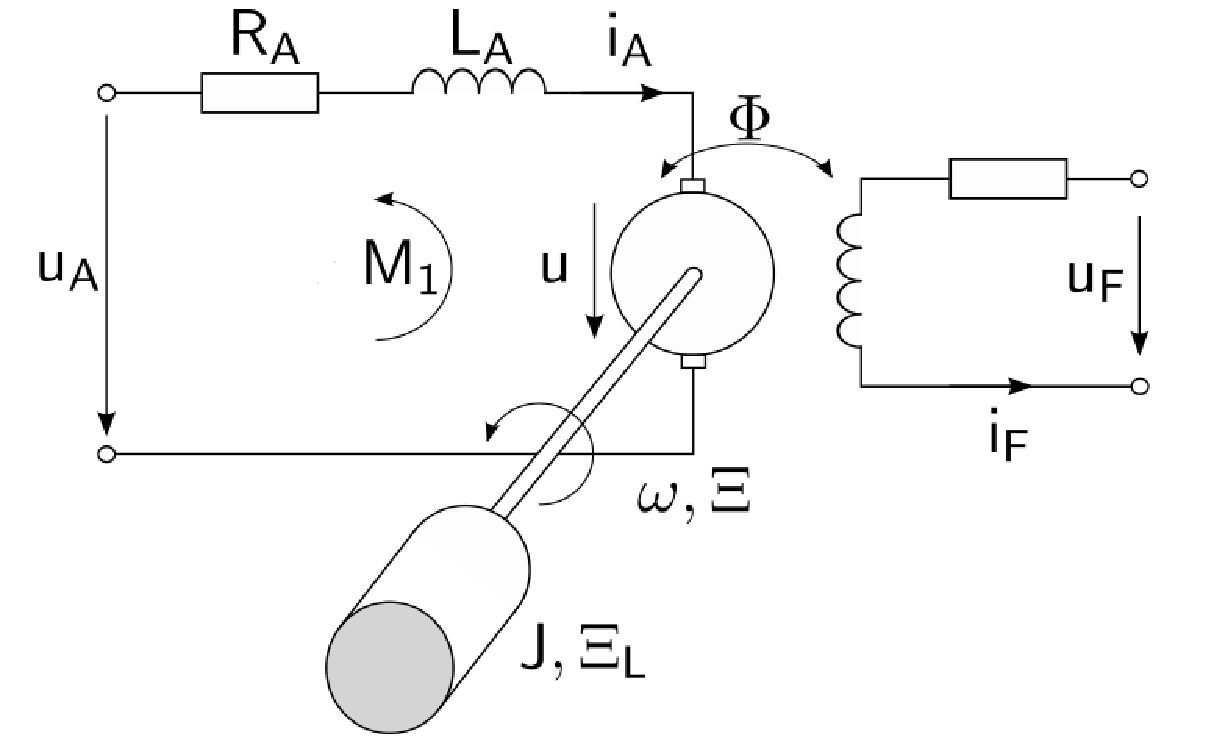
\includegraphics[width=70mm]{motor.pdf}
		\caption{Structure of the Permanent Magnet DC Motor Model. \\ \footnotesize{Source: Institut of Control Theory TU Dresden: Regelungstechnikpraktikum, Praktikumsanleitung}}
	\end{figure}
	
	%%%%%%%%%%%%%%%%%%%%%% MDOEL EQUATIONS %%%%%%%%%%%%%%%%%%%%%%%%%%%
	
	\section{Model Equations} % MUST
	
	State Vector and Input Vector:
	\begin{align*}
		\underline{x} &= (\omega \ i_A)^T &= (x_1 \ x_2)^T \\
		\underline{u} &= (u_A \ \xi_L)^T &= (u_1 \ u_2)^T \\
	\end{align*}
	
	\noindent System Equations:			
	\begin{subequations}
	\begin{align}
		\dot{x}_1 &= \frac{c\phi}{J}x_2 - \frac{1}{J}u_2 \\
		\dot{x}_2 &= -\frac{R_A}{L_A}x_2 - \frac{c\phi}{L_A}x_1 + \frac{1}{L_A}u_1
	\end{align}
	\end{subequations}

	%%%%%%%%%%%%%%%%%%%%%% PARAMETERS | OUTPUTS %%%%%%%%%%%%%%%%%%%%%%%%%%%
	\noindent
	Parameters: $c\phi, \, J, \, L_A, \, R_A$% variables with constant, predefined value
	\\
	Output: $\omega$ \\ % MAY
	

	%%%%%%%%%%%%%%%%%%%%%% EXEMPLARY PARAMETER VALUES %%%%%%%%%%%%%%%%%%%%%%%%%%%	
	
	\subsection{Exemplary parameter values}
	\begin{tabular}{cl}
\hline
  Symbol  & Value                                                                                                                                                                                \\
\hline
   $A$    & $\left[\begin{matrix}0.8189 & 0.0863 & 0.09 & 0.0813\\0.2524 & 1.0033 & 0.0313 & 0.2004\\-0.0545 & 0.0102 & 0.7901 & -0.258\\-0.1918 & -0.1034 & 0.1602 & 0.8604\end{matrix}\right]$ \\
   $B$    & $\left[\begin{matrix}0.0045 & 0.0044\\0.1001 & 0.01\\0.0003 & -0.0136\\-0.0051 & 0.0936\end{matrix}\right]$                                                                          \\
 $B_{1}$  & $\left[\begin{matrix}0.0045 & 0.0044\\0.1001 & 0.01\\0.0003 & -0.0136\\-0.0051 & 0.0936\end{matrix}\right]$                                                                          \\
 $C_{1}$  & $\left[\begin{matrix}1.0 & 0 & -1.0 & 0\\0 & 0 & 0 & 0\\0 & 0 & 0 & 0\end{matrix}\right]$                                                                                            \\
   $C$    & $\left[\begin{matrix}1.0 & 0 & 0 & 0\\0 & 0 & 1.0 & 0\end{matrix}\right]$                                                                                                            \\
 $D_{11}$ & $\left[\begin{matrix}0 & 0 & 0\\0 & 0 & 0\\0 & 0 & 0\end{matrix}\right]$                                                                                                             \\
 $D_{12}$ & $\left[\begin{matrix}0 & 0\\1.0 & 0\\0 & 1.0\end{matrix}\right]$                                                                                                                     \\
 $D_{21}$ & $\left[\begin{matrix}0 & 1.0 & 0\\0 & 0 & 1.0\end{matrix}\right]$                                                                                                                    \\
\hline
\end{tabular}

	%%%%%%%%%%%%%%%%%%%%%% DERIVATION & EXPLANATION %%%%%%%%%%%%%%%%%%%%%%%%%%%	
	
	\section{Derivation and Explanation} % SHOULD
	The function of the electrical motor is based on the interaction between the electromechanical power law and Faraday's law of induction.
	\begin{align}
		\xi (t) &= c\phi i_A(t) \\
		u(t) &= c\phi \omega(t)
	\end{align}
	The following applies to the voltage drops in the electrical armature circuit: 
	\begin{align}
		u_A(t) &= u(t) + R_A i_A(t) + L_A\frac{di_A(t)}{dt}. 
	\end{align}
	For the mechanical system, Newton's law for rotational motion provides
	\begin{align}
		\frac{\omega(t)}{dt} &= \frac{1}{J}\xi_b(t). 
	\end{align}
	Furthermore: 
	\begin{align}
		\xi_b(t) = \xi(t) - \xi_L(t). 
	\end{align}
	%%%%%%%%%%%%%%%%%%%%%% REFERENCES %%%%%%%%%%%%%%%%%%%%%%%%%%%
	
	\begin{thebibliography}{10}		
		\bibitem{But21}Institut of Control Theory TU Dresden: 
		\textit{Regelungstechnikpraktikum, Praktikumsanleitung}, published on OPAL April 2022. \\
		(not publicly accessible)
	\end{thebibliography}

\end{document}

